% PyCon US 2026 academic poster
% Breaking the Speed Limit: Fast Statistical Models with Python 3.14, Numba, and JAX

\documentclass[final]{beamer}

\usepackage[T1]{fontenc}
\usepackage{lmodern}
\usepackage[size=custom,width=120,height=72,scale=1.0]{beamerposter}
\usetheme{gemini}
\usecolortheme{imsa}
\usepackage{booktabs}
\usepackage{graphicx}
\usepackage{tikz}
\usepackage{xcolor}
\usepackage{array}

\usetikzlibrary{arrows.meta,positioning}

\definecolor{paper}{HTML}{FFF8F2}
\definecolor{ink}{HTML}{17202A}
\definecolor{muted}{HTML}{5F6B74}
\definecolor{line}{HTML}{E4D7C6}
\definecolor{cityured}{HTML}{B01117}
\definecolor{cityumaroon}{HTML}{981B49}
\definecolor{cityuorange}{HTML}{E07541}
\definecolor{cityugold}{HTML}{D99A1E}
\definecolor{numba}{HTML}{2F7D32}
\definecolor{jaxberry}{HTML}{B51E59}
\definecolor{threadteal}{HTML}{1F7A8C}
\definecolor{slideblue}{HTML}{2C6FB7}
\definecolor{softblue}{HTML}{EAF2FB}
\definecolor{softgreen}{HTML}{EAF6EA}
\definecolor{softgold}{HTML}{FFF3DC}
\definecolor{softberry}{HTML}{F8E7EF}
\definecolor{softteal}{HTML}{E8F6F5}

\setbeamercolor{background canvas}{bg=paper}
\setbeamercolor{normal text}{fg=ink}
\setbeamercolor{block title}{fg=cityured,bg=white}
\setbeamercolor{block body}{fg=ink,bg=white}
\setbeamercolor{block alerted title}{fg=cityured,bg=cityuorange!15}
\setbeamercolor{block alerted body}{fg=ink,bg=cityuorange!7}
\setbeamercolor{headline title}{fg=cityumaroon}
\setbeamercolor{headline}{fg=ink,bg=paper}
\setbeamercolor{headline rule}{bg=cityured}
\setbeamerfont{block title}{size=\Large,series=\bfseries}
\setbeamerfont{block body}{size=\large}
\setbeamerfont{headline title}{size=\Huge,series=\bfseries}

\newlength{\sepwidth}
\newlength{\colwidth}
\setlength{\sepwidth}{0.017\paperwidth}
\setlength{\colwidth}{0.290\paperwidth}
\newcommand{\separatorcolumn}{\begin{column}{\sepwidth}\end{column}}

\hyphenpenalty=10000
\exhyphenpenalty=10000
\setlength{\parindent}{0pt}
\setlength{\parskip}{0.15em}
\linespread{0.96}
\newcolumntype{L}[1]{>{\raggedright\arraybackslash}p{#1}}

\title{Breaking the Speed Limit}
\subtitle{Fast statistical models with Python 3.14, Numba, and JAX}
\author{Wenxin Jiang \textperiodcentered{} Jian Yin}
\institute[shortinst]{Department of Biostatistics, City University of Hong Kong \textperiodcentered{} PyCon US 2026}

\setbeamertemplate{headline}{
  \begin{beamercolorbox}{headline}
    \begin{columns}[c,totalwidth=\paperwidth]
      \begin{column}{0.15\paperwidth}
        \centering
        
\includegraphics[width=0.78\linewidth]{cityu_logo.pdf}
      \end{column}
      \begin{column}{0.66\paperwidth}
        \vskip0.35ex
        {\usebeamerfont{headline title}\usebeamercolor[fg]{headline title}\inserttitle\par}
        \vspace{0.25ex}
        {\Large\bfseries\color{ink}\insertsubtitle\par}
        \vspace{0.35ex}
        {\normalsize\bfseries\color{ink}Validate the statistical result first. Then accelerate the bottleneck.\par}
        \vspace{0.20ex}
        {\large\color{cityumaroon}\insertauthor\par}
        {\normalsize\color{cityured}\insertinstitute\par}
      \end{column}
      \begin{column}{0.15\paperwidth}
        \centering
        
\includegraphics[width=0.46\linewidth]{assets/repo_qr.png}\\[-0.1ex]
        {\small\bfseries\color{ink}github.com/LucaJiang/\par FastStatisticalModels4Python}
      \end{column}
    \end{columns}
    \vspace{0.75ex}
    \begin{beamercolorbox}[wd=\paperwidth,colsep=0.45ex]{headline rule}\end{beamercolorbox}
  \end{beamercolorbox}
}

\newcommand{\smalllabel}[2]{%
  {\normalsize\bfseries\color{#1}#2}\par%
}

\newcommand{\badge}[3]{%
  \noindent\fcolorbox{#1!35}{#1!8}{%
    \begin{minipage}{0.296\linewidth}
      \vspace{0.38em}
      {\large\bfseries\color{#1}#2}\par
      {\normalsize\color{ink}#3}
      \vspace{0.38em}
    \end{minipage}}%
}

\newcommand{\evidencebox}[3]{%
  \noindent\fcolorbox{#1!38}{#2}{%
    \begin{minipage}{0.94\linewidth}
      \vspace{0.35em}
      #3
      \vspace{0.35em}
    \end{minipage}}%
}

\newcommand{\toolchip}[2]{%
  \begingroup
  \setlength{\fboxsep}{0.46em}
  \colorbox{#1!12}{\large\bfseries\color{#1}#2}%
  \endgroup
}

\newcommand{\workflowrow}[3]{%
  \noindent\fcolorbox{#1!45}{#1!8}{%
    \begin{minipage}{0.94\linewidth}
      \vspace{0.18em}
      {\large\bfseries\color{#1}#2}\quad{\large #3}
      \vspace{0.18em}
    \end{minipage}}\par\vspace{0.18em}%
}

\newcommand{\practicalstep}[3]{%
  \begin{minipage}[c]{0.44\linewidth}
    \centering
    {\Large\bfseries\color{#1}#2}\par
    {\large\bfseries\color{ink}#3}
  \end{minipage}
}

\newcommand{\evidencebadge}[3]{%
  \noindent\fcolorbox{#1!35}{#1!7}{%
    \begin{minipage}{0.94\linewidth}
      \vspace{0.22em}
      {\normalsize\bfseries\color{#1}#2}\par
      {\normalsize\color{ink}#3}
      \vspace{0.22em}
    \end{minipage}}\par\vspace{0.18em}%
}

\begin{document}
\begin{frame}[t]
\vspace{0.45cm}
\begin{columns}[t,totalwidth=0.94\paperwidth]
\separatorcolumn

\begin{column}{\colwidth}
  \begin{block}{1. Why simulation is the statistical test harness}
    Real biomedical data rarely comes with ground truth. Simulation lets us know what should be recovered, calibrated, or preserved.

    \vspace{0.38em}
    \workflowrow{cityured}{Define target}{recovery / calibration / estimand}
    \workflowrow{threadteal}{Generate scenarios}{signal, dimension, hard cases}
    \workflowrow{cityuorange}{Reference first}{readable Python oracle}
    \workflowrow{numba}{Validate}{equivalence / recovery / calibration}
    \workflowrow{jaxberry}{Scale}{measure bottlenecks}

    \vspace{0.50em}
    \evidencebox{cityured}{softgold}{%
      \smalllabel{cityumaroon}{Governing rule}
      {\Large\bfseries Same question. Same result. Then faster code.}
    }
  \end{block}

  \begin{block}{2. What a statistician has to decide}
    \begin{tabular}{@{}L{0.30\linewidth}L{0.62\linewidth}@{}}
      \toprule
      \textbf{Question} & \textbf{Decision before timing} \\
      \midrule
      Scientific target & estimator, statistic, null model \\
      Ground truth & simulated labels, known effect, or nominal type-I rate \\
      Acceptance criterion & exact match, tolerance, calibration band \\
      Scale stress & $N$, $d$, $K$, $p$, $R$, workers, batch size \\
      \bottomrule
    \end{tabular}

    \vspace{0.78em}
    \badge{slideblue}{Reference}{readable oracle}
    \hfill
    \badge{threadteal}{Scenario grid}{property / stress / load tests}
    \hfill
    \badge{jaxberry}{Validation gate}{optimize only after checks}
  \end{block}
\end{column}

\separatorcolumn

\begin{column}{\colwidth}
  \begin{block}{3. Two workloads, two pressure shapes}
    They are simple examples of two common statistical computing patterns.

    \vspace{0.28em}
    \hspace*{-0.04\linewidth}\begin{columns}[t,totalwidth=1.08\linewidth]
      \begin{column}{0.49\linewidth}
        \smalllabel{numba}{k-means}
        Iterative model fitting.
        \vspace{0.15em}
        \begin{center}
          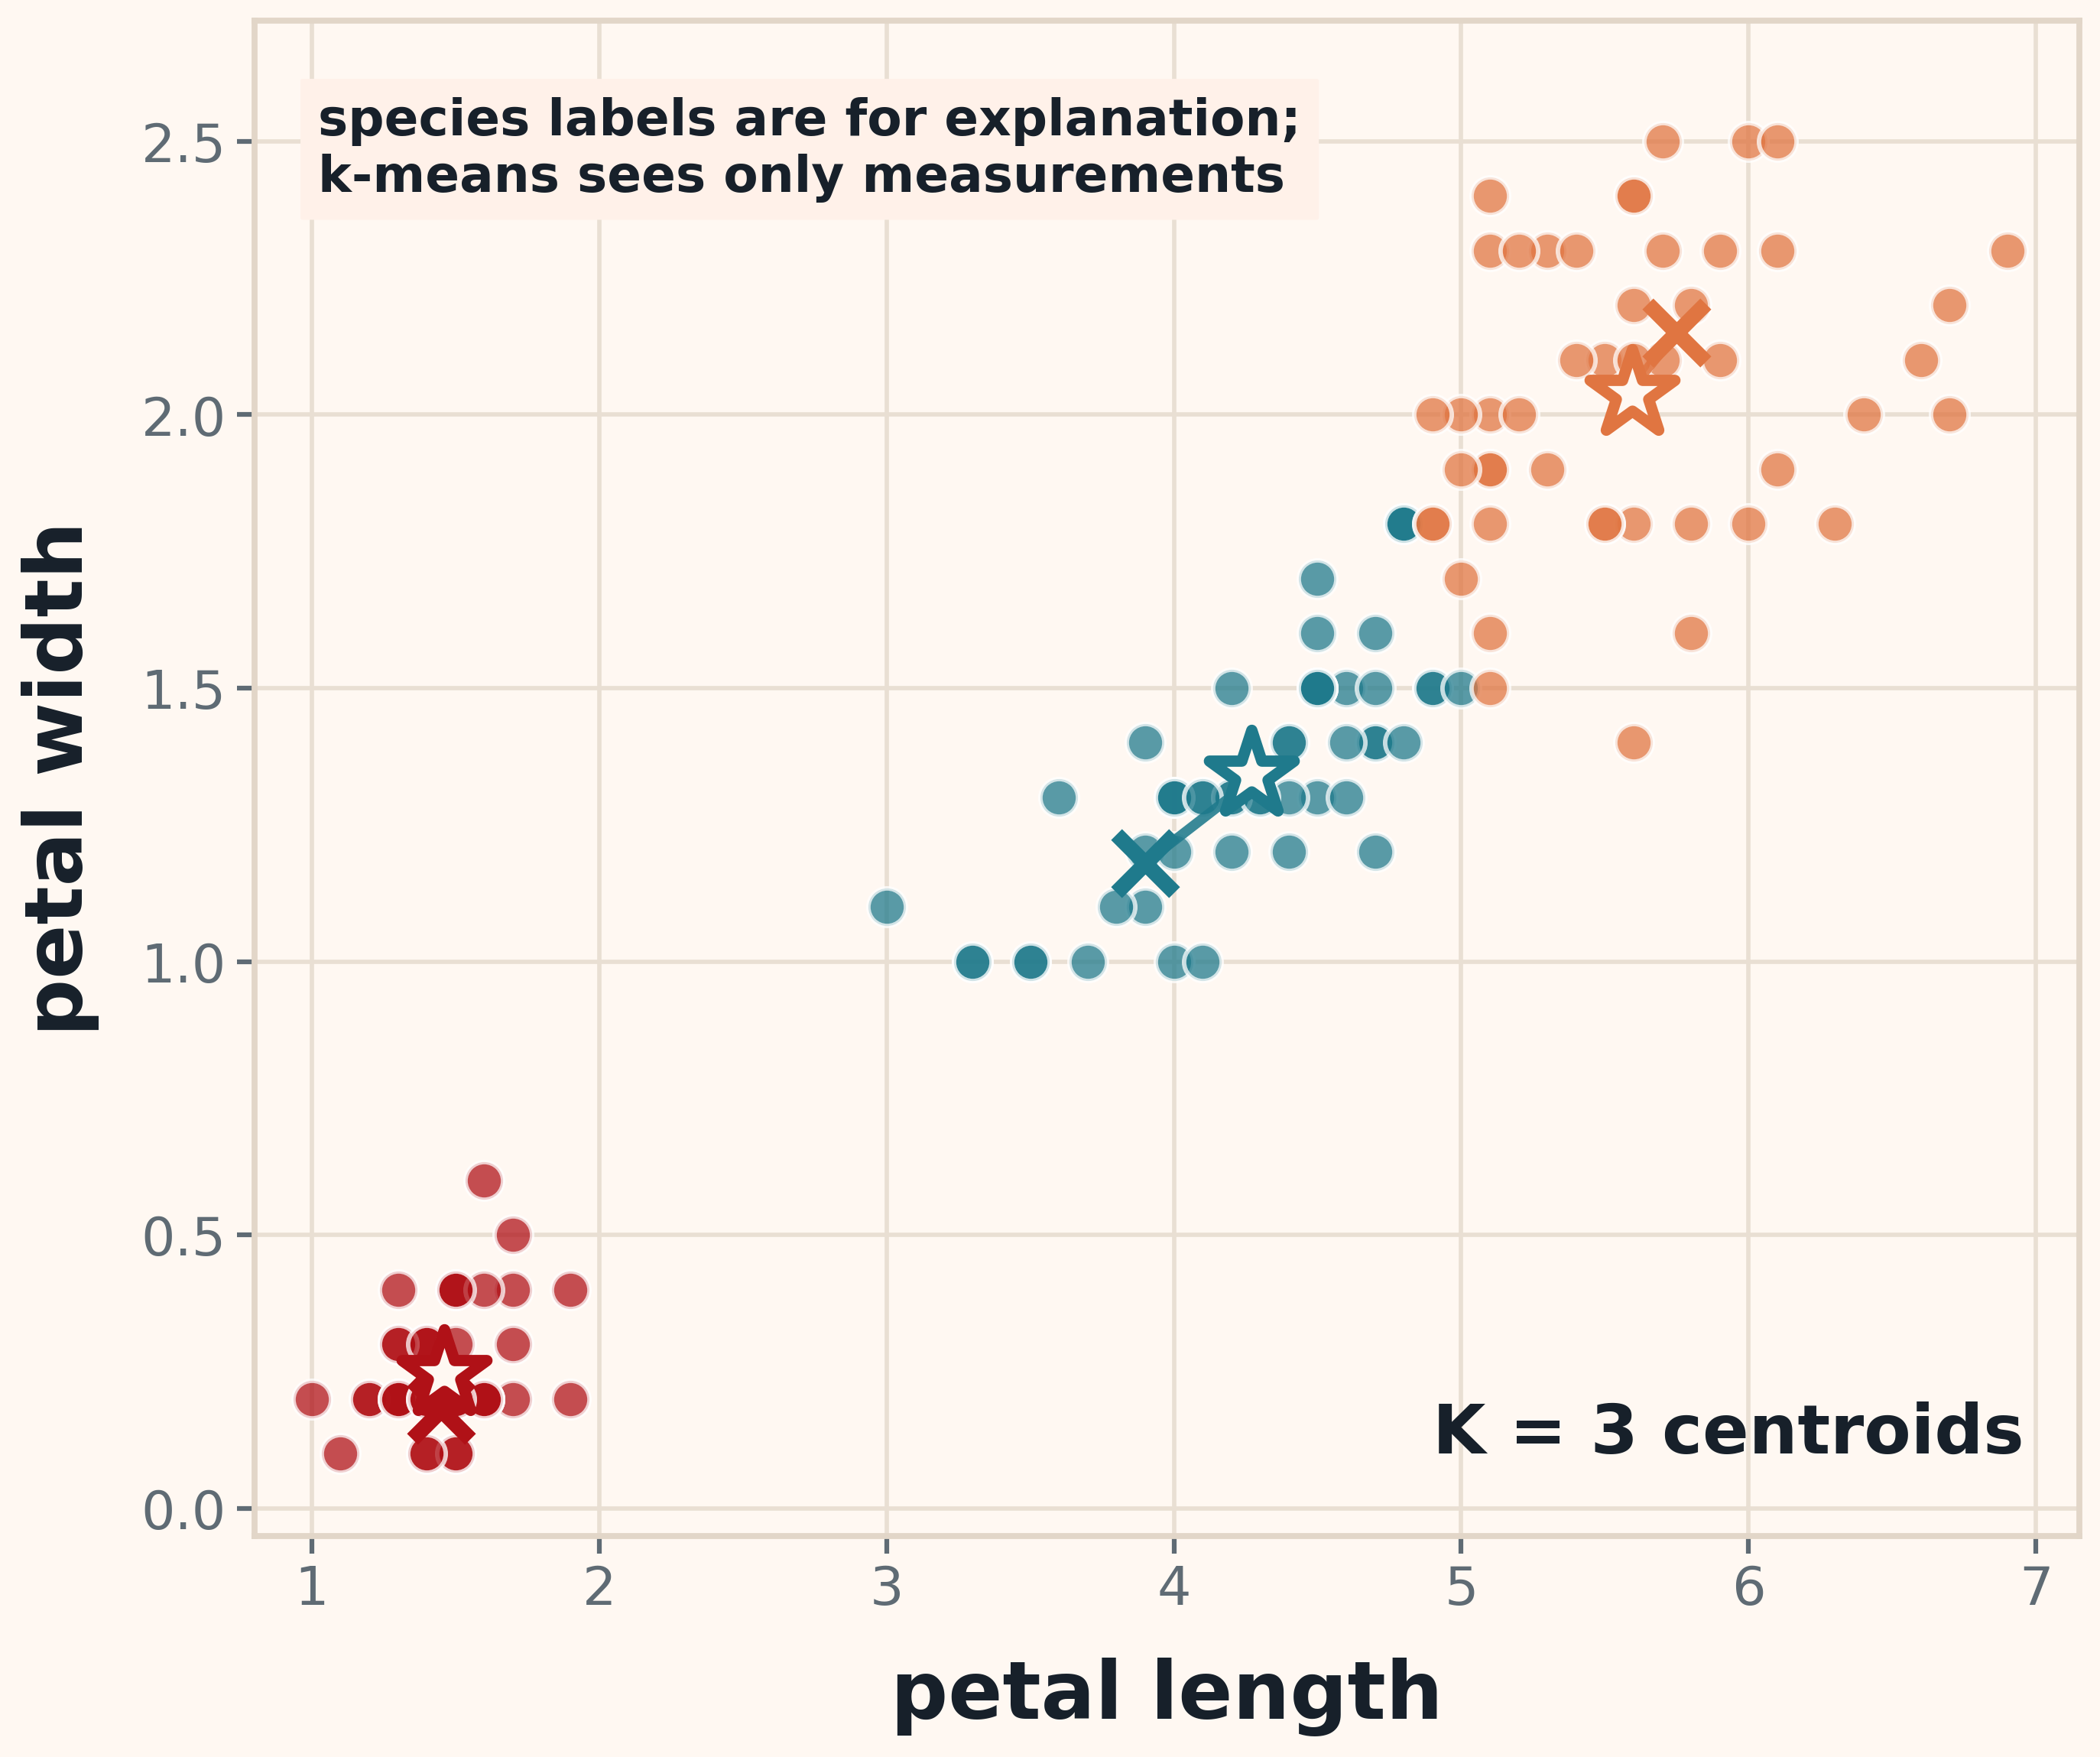
\includegraphics[width=\linewidth]{assets/poster_v4_kmeans_iris.png}
        \end{center}
      \end{column}
      \begin{column}{0.49\linewidth}
        \smalllabel{jaxberry}{permutation test}
        Resampling inference.
        \vspace{0.15em}
        \begin{center}
          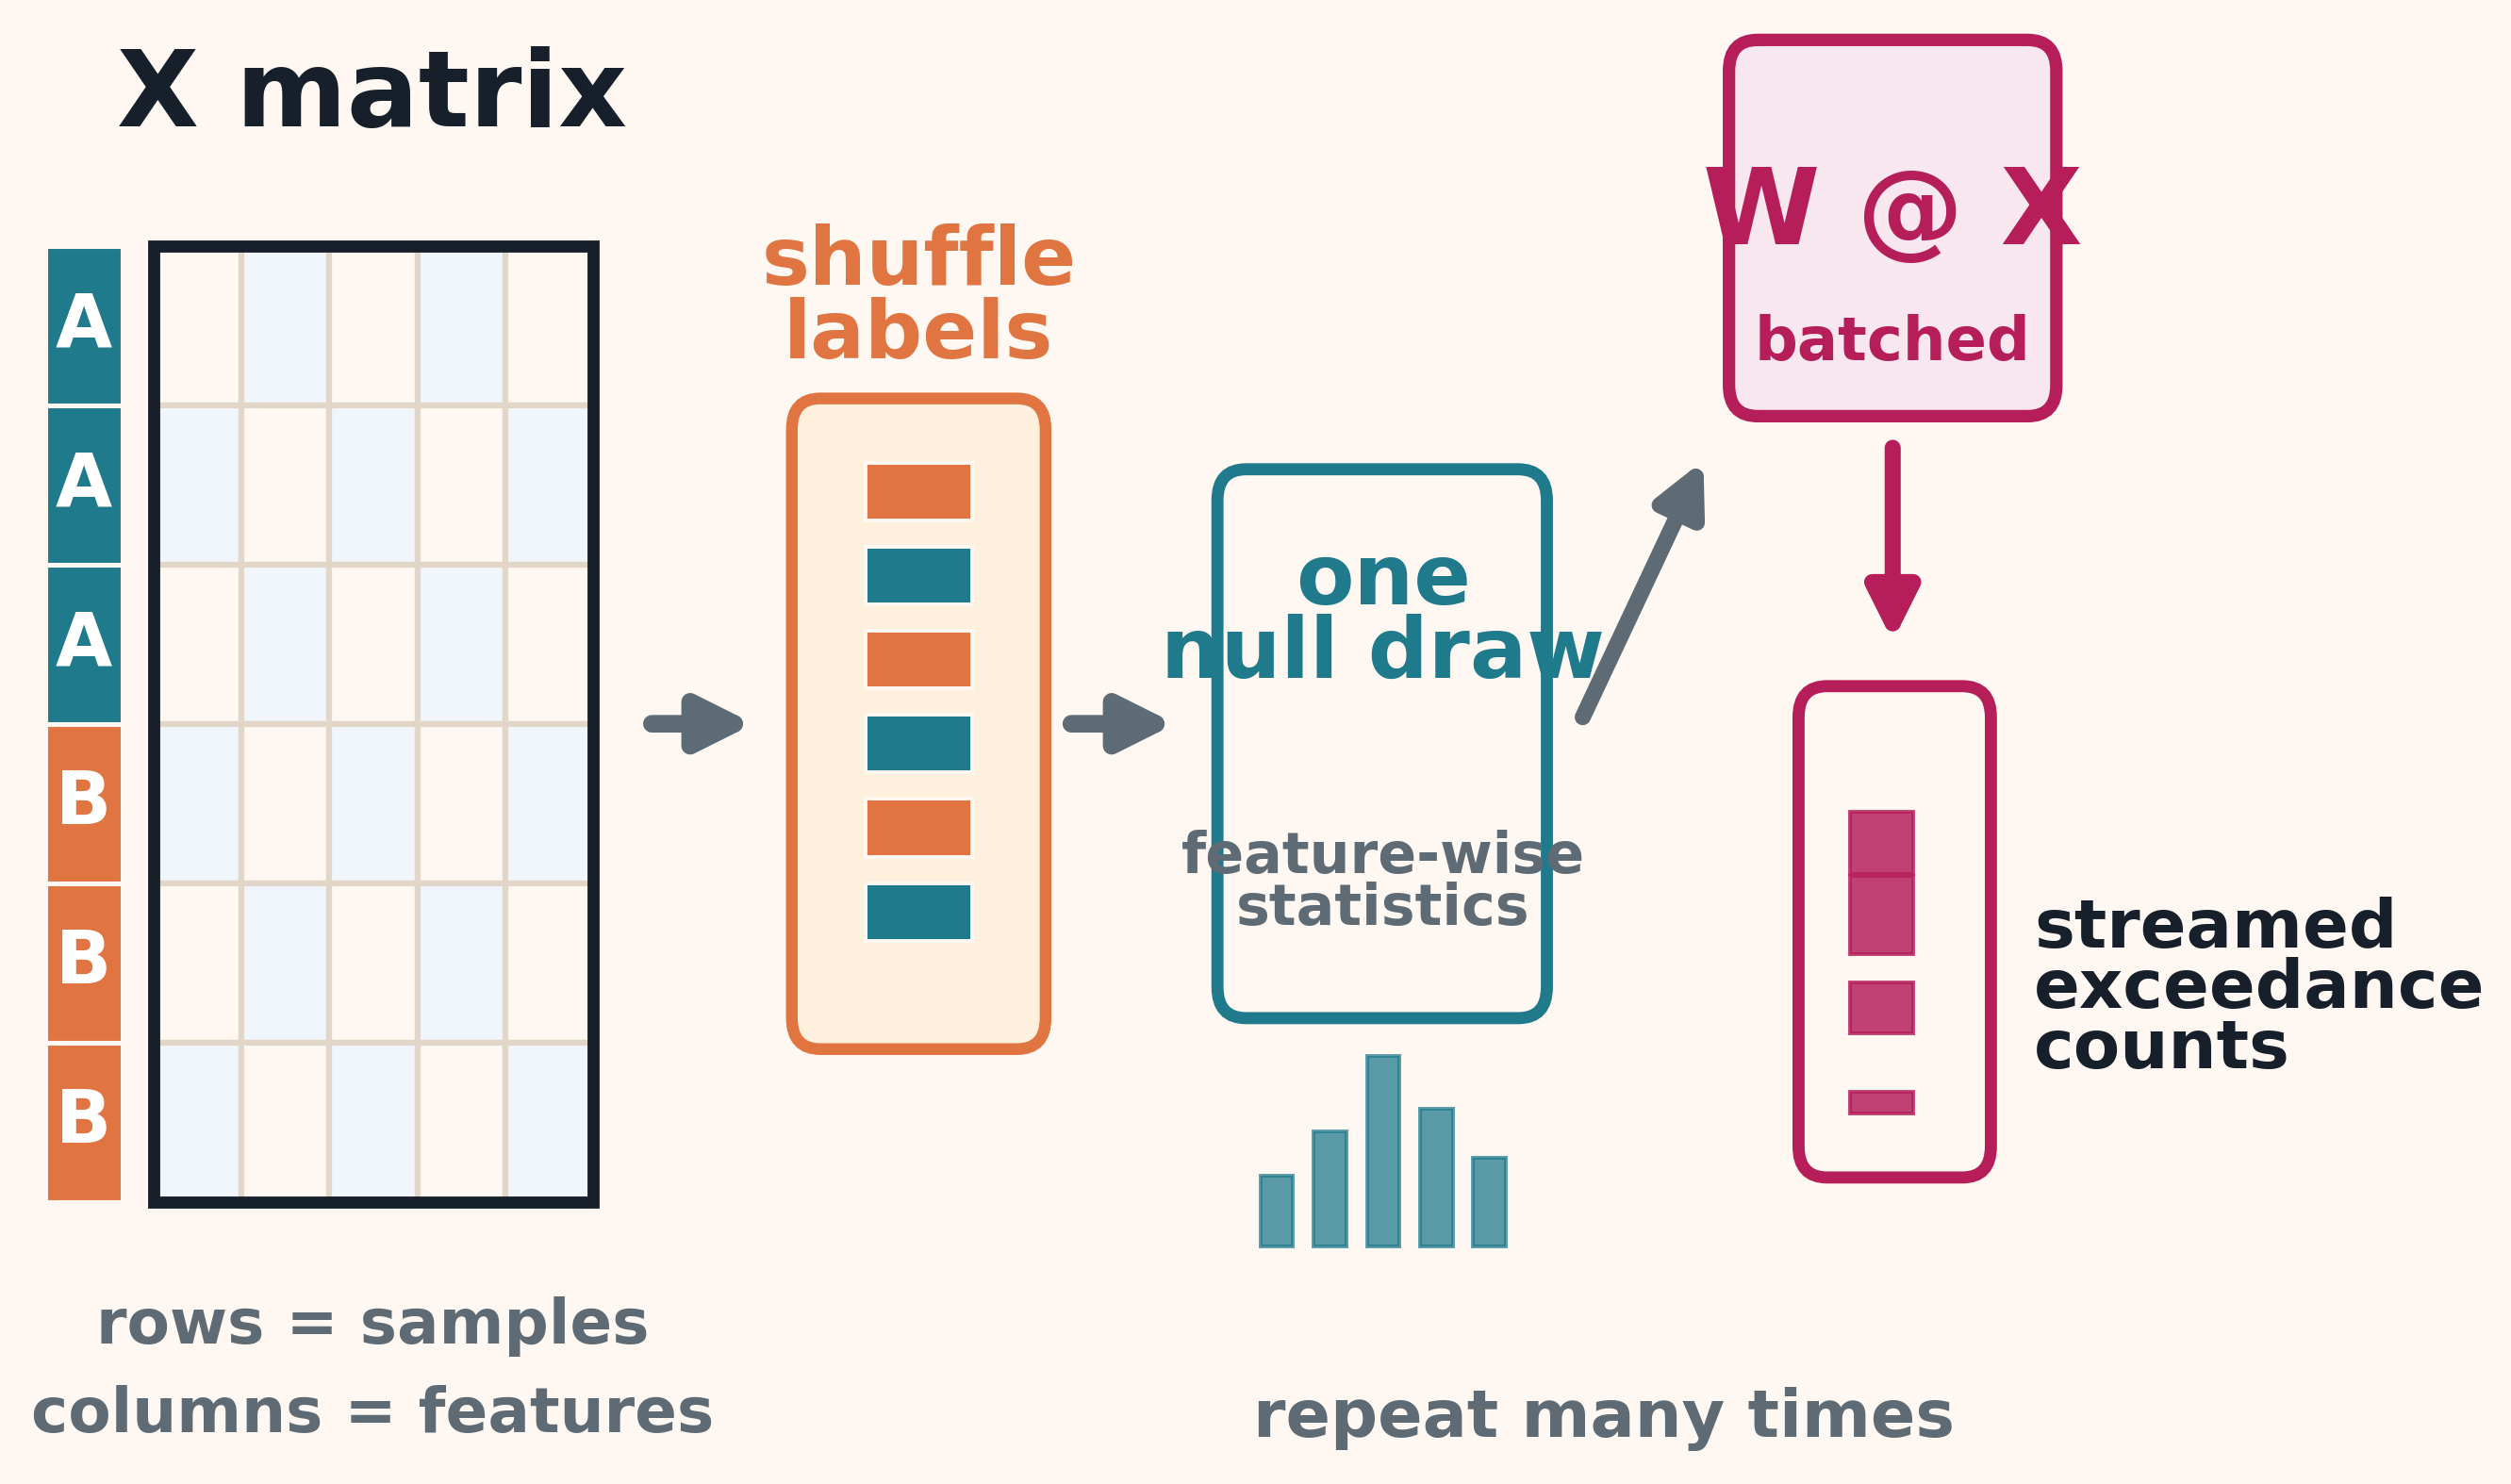
\includegraphics[width=\linewidth]{assets/poster_v6_permutation_workflow_cropped.png}
        \end{center}
      \end{column}
    \end{columns}

    \vspace{0.22em}
    \evidencebox{numba}{softgreen}{%
      \smalllabel{cityumaroon}{Validation checks}
      \textbf{k-means:} same data, initialization, stopping rule; compare inertia and recovery.\par
      \textbf{permutation:} same permutation stream and p-value definition; check null calibration before timing.
    }
  \end{block}

  \begin{block}{4. Evidence examples, scoped}
    \begin{tabular}{@{}L{0.34\linewidth}L{0.56\linewidth}@{}}
      \toprule
      \textbf{Claim} & \textbf{Committed evidence} \\
      \midrule
      k-means equivalence & max relative inertia difference $3.1\times10^{-14}$; tolerance $10^{-8}$ \\
      permutation equivalence & max p-value difference 0.0; max statistic difference $9.4\times10^{-16}$ \\
      null behavior & type-I estimate at $\alpha=0.05$ was 0.051 \\
      A100 boundary & first streamed-reduction win at $n=5{,}000$, $p=10{,}000$, $R=5{,}000$, batch\_R=8,192 \\
      A100 scope & largest slide-level measured speedup 8.54x \\
      \bottomrule
    \end{tabular}

    \vspace{0.42em}
    \evidencebox{cityuorange}{softgold}{%
      \smalllabel{cityumaroon}{Timing scope}
      speedup = matched CPU matrix baseline / A100 streamed full end-to-end\par
      compile excluded \textperiodcentered{} transfer included \textperiodcentered{} kernel-only excluded
    }
  \end{block}
\end{column}

\separatorcolumn

\begin{column}{\colwidth}
  \begin{block}{5. Choose the smallest tool}
    \begin{tabular}{@{}L{0.37\linewidth}L{0.51\linewidth}@{}}
      \toprule
      \textbf{Signal} & \textbf{Conservative tool choice} \\
      \midrule
      not trusted yet & fix method / reference \\
      hot scalar loop & Numba \\
      dense algebra & NumPy / BLAS \\
      shared-array repetition & Python 3.14 / threads \\
      device-resident batches & JAX / A100 \\
      giant temporary & rewrite / stream \\
      \bottomrule
    \end{tabular}

    \vspace{0.78em}
    \toolchip{cityured}{trust first}
    \hfill
    \toolchip{numba}{compile loops}
    \hfill
    \toolchip{slideblue}{use algebra}
    \hfill
    \toolchip{jaxberry}{batch for device}
  \end{block}

  \begin{block}{6. What to report with every speed claim}
    \begin{itemize}
      \item validation target and acceptance tolerance
      \item environment tier: local, server CPU, or A100
      \item cold vs warm timing; compile excluded or included
      \item transfer, allocation, and collection included or excluded
    \end{itemize}
    {\footnotesize\color{muted}Unavailable/OOM cells are reported as unavailable.}
  \end{block}

  \begin{alertblock}{Takeaway}
    \centering
    \practicalstep{cityured}{1}{Simulate known behavior}
    \hfill
    \practicalstep{threadteal}{2}{Validate the result}
    \vspace{0.55em}\par
    \hfill
    \practicalstep{cityuorange}{3}{Measure the bottleneck}
    \hfill
    \practicalstep{jaxberry}{4}{Choose the smallest tool}
    \vspace{0.55em}

    {\Large\bfseries\color{cityumaroon}Clear enough to trust. Fast enough to scale.}\par
    \vspace{0.25em}
    {\normalsize\bfseries\color{ink}github.com/LucaJiang/FastStatisticalModels4Python}
  \end{alertblock}
\end{column}

\separatorcolumn
\end{columns}
\end{frame}
\end{document}
